\documentclass{article} 
\usepackage[spanish, activeacute]{babel} %activeacute permite que podamos hacer los acentos asi nomas ''sin tener que agregarle \

%encabezado con imagen
\usepackage{fancyhdr}
\usepackage{graphicx}
\usepackage{vmargin}
\usepackage{amsmath, amsthm, amsfonts}
\usepackage{enumerate}
\usepackage{multicol}
\usepackage[table,xcdraw]{xcolor}
\usepackage{float}

% Teoremas (el estilo por defecto es plain rotulos en negrita y letra italica)
%--------------------------------------------------------------------------
\newtheorem{thm}{Teorema}[section]
\newtheorem{cor}{Corolario}[section]
\newtheorem{lem}{Lema}
\newtheorem{p}{Proposici\'on}[section]
\newtheorem{solution}{Soluci\'on}[section]

%\newtheorem{prop}[thm]{Proposici�n}
\newtheorem{prop}{Proposici\'on}[section]
%\theoremstyle{definition} %rotulo en negrita pero texto normal
\newtheorem{defn}[thm]{Definici�n}
%\theoremstyle{remark} %rotulo italica y texto normal
%\newtheorem{rem}[thm]{Observaci�n}
\newtheorem{ejem}{Ejemplo}[section]
\newtheorem{ejer}{Problema}[section]

\title{
\begin{center}

\includegraphics[width=120px, height=40px]{omapa.jpg}\\
\end{center}
}
%\author{Alberto$^1$, Mar\'ia$^2$ \\ $^1$ Universidad don bosco, $^2$ Universidad Una}
\date{}

\lhead{\begin{picture}(0,0) \put(0,0){
\includegraphics[width=20mm]{omapa.jpg}} \end{picture}}
\rhead{Nivel Pre-Avanzado}
\chead{Teor\'ia de n\'umeros}
%%\chead{\vspace{-0.3cm} Teor\'ia de n\'umeros \vspace{0.3cm}}
\renewcommand{\headrulewidth}{0.5pt}

\pagestyle{fancy}

\begin{document}
\maketitle
\begin{center}
\bfseries{Curso de Iniciaci'on Cient'ifica para J'ovenes Talentos\\
Nivel Pre-Avanzado \\
}
\end{center}

\begin{center}
	{\bfseries {\Large Coloraciones en Olimpiadas}}
\end{center}

La coloraci\'on en las Matem\'aticas es un tema de relevancia considerable. La idea es clasificar una colecci\'on de objetos en conjuntos con caracter\'isticas parecidas, vali\'endonos de la facilidad que tiene nuestro cerebro para identificar colores. 

Generalmente se colorean tableros, aunque eventualmente planos o puntos pueden ser susceptibles al m\'etodo.



\section{El tablero de Ajedrez}

En 1961, un F\'isico Te\'orico Brit\'anico llamado M. Fischer resolvi\'o un problema de tableros famoso de la \'epoca: ¿De cu\'antas formas es posible colocar $32$ domin\'os de $2\times 1$ en un tablero de ajedrez de $8\times 8$?. La respuesta que obtuvo es $12,988,816$ formas. 
Ahora, ¿Que sucede que cortamos dos casillas de esquinas opuestas?

\begin{ejem}
	 ¿De cu\'antas formas podemos poner $31$ domin\'os en el nuevo tablero?
\end{ejem}
\begin{proof}
	Este problema parece considerablemente m\'as dif\'icil que el que resolvi'o M. Fischer, a simple vista. Sin embargo, ese no es el caso. Consideremos el tablero de Ajedrez, pintado en blanco y negro de manera alternada. Las dos casillas recortadas son del mismo color (pueden ser negras o blancas, pero siempre del mismo color). Por lo tanto de las $64$ casillas, hay $32$ de un color y $30$ de otro color. 
	
	Primero observemos que cada domin\'o cubre exactamente una casilla negra y una blanca. Suponiendo que el tablero pueda cubrirse con esas $31$ piezas, entonces deber\'ia haber $31$ casillas de cada color. Pero eso no ocurre. Concluimos entonces que es imposible cubrir el nuevo tablero con $31$ piezas de domin\'o. 
\end{proof}
 

Existen dos observaciones importantes que se pueden rescatar de \'esta prueba. 
\begin{enumerate}
	\item Podemos encontrarnos en dos situaciones diferentes en problemas de colocar piezas en tableros: O es posible cubrir el tablero o no. En el primer caso, es suficiente con encontrar una configuraci\'on para concluir que es posible, pero notemos que para concluir que es \textbf{imposible} cubrir el tablero, deber\'iamos mostrar que \textbf{ninguna} configuraci\'on funciona. Esto \'ultimo generalmente no es el camino correcto. Se necesita de una idea inteligente para atacar el problema. Una idea posible es la coloraci\'on.
	\item Existe una receta que ayuda\footnote{¡Ninguna t\'ecnica solucionar\'a todos los problemas!} a resolver muchos problemas de \'este tipo:
	\begin{enumerate}[a.]
		\item Colore\'a el tablero de una forma que te parezca \'util (Ajedrez). %Porque es util?
		\item Encontr\'a una propiedad que te d\'e la coloraci\'on (Cada domin\'o cubre exactamente una casilla de cada color). 
		\item Supon\'e que la hip\'otesis es falsa, y lleg\'a a una contradicci\'on (Deber\'ia haber $31$ casillas de cada color, pero eso no pasa).
	\end{enumerate}

	
	
\end{enumerate}

Veamos esta receta en acci\'on

\begin{ejem} \label{ejemplotetramino}
	Decidir si es posible cubrir completamente\footnote{A menos  que se especifique lo contrario, no se est\'a permitido de superponer las piezas ni salirse del tablero, pero podemos rotar y girar las piezas.} un tablero de $10 \times 10 $ con piezas iguales al de la figura.
\end{ejem}
\begin{proof}
	Lo primero es lo primero: intentar cubrir el tablero con las piezas indicadas. Luego de unos intentos fallidos, nuestra intuici\'on probablemente nos diga que no es posible cumplir el cometido. Es ah\'i cuando empezamos a poner las manos en la masa:
	
	\begin{enumerate}[a.]
		
		\item \textit{Colore\'a el tablero}
		
		El segundo ejemplo no puede ser diferente al primero, necesitamos empaparnos de esta nueva t\'ecnica: Coloreamos el tablero como un tablero de ajedrez. Esta parte ya la conocemos.
		
		\item \textit{Encontrar una propiedad en la coloraci\'on.}
		
		Podemos observar que, no importa donde se coloque la pieza, siempre estar\'a sobre tres casillas del mismo color y una casilla del color diferente. Es decir, cualquier pieza que se coloque sobre el tablero ocupar\'a una cantidad impar de casillas blancas. Adem\'as, $50$ de las $100$ casillas del tablero son blancas.
		
		\item \textit{Supongamos que la hip\'otesis es falsa}
		
		Es decir, es posible cubrir el tablero completamente, para lo cual necesitaremos $\frac{100}{4} = 25$ piezas. La observaci\'on clave es combinar los dos \'ultimos datos. Estas $25$ piezas cubrir\'an indefectiblemente una cantidad impar (suma de una cantidad impar de n\'umeros impares) de casillas blancas, pero hay $50$ casillas blancas, el cual es un n\'umero par. Luego, es imposible cubrir el tablero.
	\end{enumerate}
\end{proof}

\subsection{Problemas}

\begin{enumerate}
	\item En un sal\'on de clase est\'an sentados los alumnos formando un arreglo rectangular de 5 $\times$ 7. La maestra
	que quiere hacer una din\'amica, les pide a todos los alumnos que intercambien de lugar con un compañero
	vecino, movi\'endose un lugar ya sea a la izquierda, a la derecha, adelante o atr\'as de su lugar. Pepito, que
	sabe de matem\'aticas, le dice a la maestra que esto es imposible. ¿Por qu\'e tiene raz\'on Pepito?
	\item Un rat\'on se quiere comer una pila de cubitos de queso de $5\times5\times5$ y quiere ir comiendo cada cubito iniciando por un cubito de la orilla y
	terminando en el cubito central. Adem\'as, cada que come un cubito, el siguiente cubito que se come es uno
	de los adyacentes (no en diagonal). ¿Podr\'a el rat\'on comerse el queso de esta manera?
	
	\item El ejemplo \ref{ejemplotetramino} muestra el problema de cubrir un tablero de $10\times 10$ con un tetramin\'o (una pieza que se compone de cuatro casillas). Existen otros cuatro tipos de tetramin\'os (Si, esos que aparecen en el tetris). Analice cada caso: ¿Es posible cubrir el tablero $10\times 10$
	
	\item Una tripleta ordenada de n\'umeros enteros positivos $(a, b, n)$ es dicha \textit{veraniega} si es posible cubrir un cuadrado de $n \times n$ con piezas de tamaño $a\times b$. Halle la cantidad de tripletas \textit{veraniegas} de la forma $(a, b, n)$, donde $n$ equivale al año en el cual nos encontramos.
\end{enumerate}

\section{Otras coloraciones}

No todos los problemas se resuelven colorando como tablero de ajedrez. Veamos unos ejemplos.

\begin{ejem}
	Decidir si es posible cubrir completamente un tablero de $10 \times 10 $ con tetramin\'os iguales al de la figura siguiente
	\begin{figure}[h!]
		\centering
		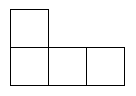
\includegraphics[scale=.8]{imgs/color4.png}
	\end{figure}
\end{ejem}

\begin{proof}
	Empecemos observando que la coloraci\'on de ajedrez no ayuda mucho. Cada ficha subre exactamente dos casillas blancas y dos casillas negras, y hay $50$ casillas blancas y $50$ casillas negras.
	
	Es importante notar que si una coloraci\'on no sirve, ¡Eso no implica que no haya otra coloraci\'on que si sirva!. Apliquemos entonces una vez mas nuestra receta:
	
	\begin{enumerate}[a.]
		
		\item \textit{Colore\'a el tablero}
		
		Para este problema, vamos a colorear las columnas de del tablero de blanco y negro, de manera alternada.
		
		\item \textit{Encontrar una propiedad en la coloraci\'on.}
		
		Podemos observar que, no importa donde se coloque la pieza, siempre estar\'a sobre tres casillas del mismo color y una casilla del color diferente. Es decir, cualquier pieza que se coloque sobre el tablero ocupar\'a una cantidad impar de casillas blancas. Adem\'as, $50$ de las $100$ casillas del tablero son blancas.
		
		\item \textit{Supongamos que la hip\'otesis es falsa}
		
		Es decir, es posible cubrir el tablero completamente, para lo cual necesitaremos $\frac{100}{4} = 25$ piezas. La observaci\'on clave es combinar los dos \'ultimos datos. Estas $25$ piezas cubrir\'an indefectiblemente una cantidad impar (suma de una cantidad impar de n\'umeros impares) de casillas blancas, pero hay $50$ casillas blancas, el cual es un n\'umero par. Luego, es imposible cubrir el tablero.
	\end{enumerate}
\end{proof}

El ojo experto seguro habr\'a notado que \'esta soluci\'on se parece mucho a la del ejemplo \ref{primerejemplo}. No es coincidencia: La virtud de un buen matem\'atico es el saber adaptar soluciones ya vistas a los nuevos desaf\'ios que se le presentan.

\begin{ejem}
	A un tablero de $8 \times 8$ se le ha recortado una casilla de una de las esquinas. Decidir si es posible cubrirlo completamente con fichas de tamaño $3 \times 1$.
\end{ejem}

\begin{proof}
	
	Ya no es ning\'un secreto a la altura de este folleto, vamos a usar la receta:
	
	
	\begin{enumerate}[a.]
		
		\item \textit{Colore\'a el tablero}
		
		Observemos la siguiente coloraci\'on:
		
		\begin{figure}[h!]
			\centering
			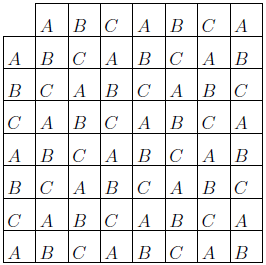
\includegraphics[scale=.85]{imgs/color5.png}
		\end{figure}
		
		\item \textit{Encontrar una propiedad en la coloraci\'on.}
		
		El encanto de \'esta coloraci\'on no es otro sino el siguiente: Cada ficha cubre exactamente una casilla de cada color. 
		
		\item \textit{Supongamos que la hip\'otesis es falsa}
		
		Si el tablero pudiese cubrirse con fichas de $3 \times 1$, entonces deber\'a haber la misma cantidad de casillas de cada color. Eso no ocurre; luego no es posible cubrir el tablero. 
	\end{enumerate}
\end{proof}


Desde luego, las coloraciones que hemos visto no resolver\'an todos los problemas, siempre debemos dejar fluir nuestra imaginaci\'on.

\subsection{Problemas}

\begin{enumerate}
	\item Tenemos un tablero de $7 \times 7$ del cual le hemos recortado una esquina. ¿Es posible cubrirlo con 12 domin\'os verticales y 12 domin\'os horizontales?
	
	\item ¿Cu\'al es la mayor cantidad de casillas que se pueden colorear en un tablero de $7 \times 7 $ de manera que cada subtablero de $2 \times 2$ tiene a lo m\'aximo dos casillas pintadas?
	
	\item Decidir si es posible cubrir completamente un tablero de $10 \times 10$, sin huecos ni superposiciones y sin salirse del tablero, con fichas rectangulares de $1 \times 4$. (Cada ficha debe cubrir exactamente cuatro casillas del tablero.)
	
	\item En cada casilla de un tablero de $12 \times 12$ est\'a escrito un $1$ o un $0$. Una operaci\'on permitida es elegir $5$ casillas consecutivas en direcci\'on vertical, horizontal o diagonal, y con esas $5$ casillas cambiar cada $0$ por $1$ y cada $1$ por $0$. Inicialmente todas las casillas tienen un $0$ escrito en ellas. Determinar si es posible, mediante una secuencia de operaciones permitidas, lograr que todas las casillas del tablero tengan un $1$.
	
	\item Tengo un cuarto cuyo piso tiene forma rectangular y est\'a totalmente cubierto por piezas de azulejos de tamaño $2 \times 2$ y $1\times 4$. Una de las piezas de tamaño $1\times 4$ se ha roto, y solo me queda una pieza de tamaño $2\times 2$ en el dep\'osito. Decidir si es posible reorganizar las piezas que tengo para cubrir completamente mi cuarto de azulejos.
	
	\item Un tablero de $7 \times 7$ se ha cubierto con la m\'axima cantidad posible de fichas de tamaño $3\times 1$. Sin embargo, siempre sobra una casilla. Determine la cantidad de lugares donde esta casilla sobrante puede ubicarse en el tablero.
	
	\item Se tiene un tri\'angulo equil\'atero de lado 7, que est\'a dividido en 49 tri\'angulitos iguales mediante rectas paralelas a sus lados. Se van recortando paralelogramos de per\'imetro 6 formado por cuatro tri\'angulitos de la grilla. Determine la mayor cantidad de paralelogramos que se pueden recortar.
	
	\item Ana y Beto juegan en un tablero de $11$ filas y $9$ columnas. Primero Ana divide el tablero en $33$ zonas. Cada zona tiene la forma de una casilla de tamaño $3\times 1$. 
	
	Luego, Beto escribe en cada casilla uno de los n\'umeros $0, 1, 2, 3, 4, 5$ de modo que la suma de los n\'umeros de cada zona sea igual a 5. Beto gana si la suma de los n\'umeros escritos en cada una de las 9 columnas del tablero es un n\'umero primo. En caso contrario, Ana gana. Demuestre que Beto tiene estrategia ganadora. 
	
	\item Se tiene un tablero de $10\times 4$, en el cual se tiene un caballo en la esquina inferior izquierda. Muestre que no es posible que el caballo realice un ciclo sobre el tablero. Es decir, no puede hacer un recorrido que visite cada casilla exactamente una vez y volver a la casilla de inicio.
	
	\item A un tablero de $n\times n$ se le ha recortado las cuatro esquinas. Determine para que valores de $n$ es posible cubrirlo completamente con tetramin\'os en forma de L.
\end{enumerate}

%\section{Coloraci\'on m\'as all\'a de los tableros}

Es un hecho de que colorear tableros es bastante \'util. Sin embargo, coloraciones en otras situaciones tambi\'en pueden ser bastante \'utiles. Es cuesti\'on de reconocer cu\'ando la situaci\'on es id\'onea para la coloraci\'on e intentarlo. Desde luego, como ya no se tratan de tableros en esta vuelta, nuestra amada receta deber\'a ser adaptada o descartada en todo caso.

\subsection{Problemas}

\begin{enumerate}
	\item Pruebe que dados $n>5$ puntos en el plano, de los cuales no hay tres colineales, es posible colorearlos de dos colores de manera que no exista una linea que separe los puntos de un color a los puntos del otro color (la l\'inea no puede pasar por ningun punto).
	
	\item Se tiene un c\'irculo dividido en $6$ sectores iguales y se escriben los n\'umeros 1, 0 1, 0, 0, 0, uno en cada secci\'on de manera ordenada. Si un movimiento consiste en sumar o restar $1$ a dos secciones adyacentes, ¿Se puede llegar, despu\'es de una cantidad finita de movimientos, a tener todas las secciones del c\'irculo con un  mismo n\'umero?.
	
	\item Se tiene un pa\'is con ciudaddes conectadas como en la figura siguiente:
	\begin{center}
		\begin{figure}[h!]
			\centering
			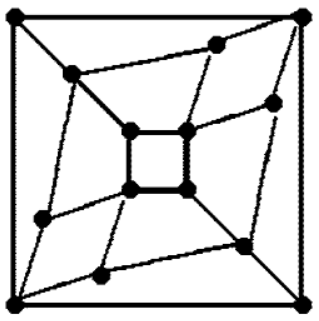
\includegraphics[scale=.5]{imgs/cities.png}
		\end{figure}
	\end{center}
	Deterimne si es posible visitar todas las ciudades exactamente una vez.
	
	\item Pruebe que es imposible dibujar un camino con el l\'apiz de maera que intersecte a todos los segmentos de la figura exactamente una vez (y no se est\'a permitido pasar por las esquinas).
	\begin{center}
		\begin{figure}[h!]
			\centering
			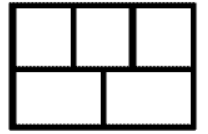
\includegraphics[scale=.4]{imgs/curve.png}
		\end{figure}
	\end{center}
	
	\item Cada punto del plano se pinta de rojo o azul. Demuestre que existen tres puntos del mismo color, de modo que uno de los puntos es el punto medio del segmento formado por los otros dos puntos
	
	\item Determine si es posible pintar cada uno de los enteros de rojo, azul o verde, de manera que se cumplan las siguientes condiciones:
	\begin{enumerate}[a.]
		\item Existe al menos un n\'umero de cada color.
		\item Si $ a+b = c$, y $a$ y $b$ son de colores diferentes, entonces $c$ es de color rojo.
	\end{enumerate}
	
	\item Se pintan los enteros positivos de negro o blanco, de manera que la suma de dos n\'umeros de diferentes colores es blanca y el producto es negro. 
\end{enumerate}
%\input{section4.tex}
%\input{section5.tex}

\begin{thebibliography}{99}


\bibitem{Engel} Engel, Arthur. \emph{Problem-Solving Strategies}, Problem books in mathematics, Springer (1998).
\bibitem{Saucedo} Saucedo, Mat\'ias. \emph{Coloracionnes en Tableros}, Folleto de Entrenamiento Cono Sur 2015 para el equipo Argentino (2015).
\bibitem{Favela} Favela, \emph{Coloraci\'on I $\&$ II}, Olimpiada Mexicana de Matem\'aticas en Baja California (2016).


\end{thebibliography}



\end{document}
